\documentclass{article}
\usepackage[utf8]{inputenc}
\usepackage{amsmath}
\usepackage{graphicx}
\usepackage{esint}

\title{Reporte de actividades semestre Marzo a Septiembre 2022}
\author{Julio César Pérez Pedraza}
\date{Agosto de 2022}

\begin{document}

\maketitle

\section{Introducción}

Para el desarrollo de este proyecto,  \textit{Propiedades de Transporte en Grafeno Pristino, Deformado y Bajo la Influencia de Campos Externos}, como se ha reportado en los previos semestres, se han estudiado diferentes herramientas teóricas y computacionales tales como el método de lattice Boltzmann clásico (LBM), el lenguaje de programacion C para su implementación computacional, la adaptación del LBM al caso relativista (RLBM) en 3D, así como la adaptación al caso 2D. Se lograron implementar algunas simulaciones sobre el flujo electrónico en el sistema del grafeno pristino, además de sistemas de grafeno con una y varias impurezas circulares, en los cuales se puede variar tanto sus radios como sus posicionamientos. De dichas simulaciones se lograron obtener perfiles de velocidad de los portadores de carga en el sistema, además de algunas propiedades de transporte del sistema tales como la conductividad y la fuerza de arrastre ($F_D$), así como las Transformadas Rápidas de Fourier (FFT) de dichas cantidades. Posteriormente, el semestre anterior se comenzó con el estudio de Inteligencia Artificial (AI), en particular, el estudio de redes neuronales (NNs). Para esto se adquirieron conocimientos del lenguaje de programación Python, el cual es de utilidad para la implementación de NNs en la plataforma TensorFlow descrita previamente.\\

Siguiendo con el plan de trabajo marcado, durante el periodo que comprende el presente reporte se procedió a implementar NNs sobre el sistema de nuestro interés. En la sección 2, se da una breve introducción a los aislantes topológicos, en particular al modelo de Shockley, para el cual se implementó un par de redes NNs y el cual utilizamos como un modelo de aprendizaje antes de comenzar a desarrollar NNs en nuestro sistema de grafeno com impurezas. Posteriormente, en la sección 3 se presentan varios modelos de NNs para nuestro sistema. En la sección 4 se menciona el trabajo que se está desarrollando actualmente, así como el trabajo a futuro que se planea realizar. Finalmente, se comenta acerca de otras actividades que se llevaron a cabo durante este periodo.

\section{Implementación de NNs en el modelo de Shockley de aislantes topológicos}
Basando nuestra discusión en las referencias [1,2], el descubrimeinto del efecto Hall cuántico en 1980 mostró que la simple división de la teoria de bandas para conducción electrónica en aislantes y metales no es el fin de la historia. En dicho efecto, aplicar un campo magnético externo sobre un metal confina el movimiento de los electrones en el bulto (\textit{bulk}), pero el mismo campo los forza hacia estados de borde (\textit{edge}) deslocalizados en la superficie. En los últimos 20 años el progreso teórico en este tipo de sistemas ha mostrado que no es necesario un campo magnético externo para tener un aislante con estados de borde conductores robustos, sino que la topología no trivial de las bandas ocupadas es el ingrediente crucial. Un aislante topológico es un material que tiene la propiedad de ser conductor en su superficie y aislante en su interior, dicha característica se debe justamente a las propiedades topológicas de la función de onda cuántica de los electrones. A pesar de que la superficie de estos materiales es conductora, el comportamiento de este difiere de los metales convencionales, pues sus electrones obedecen una dinámica análoga a partículas relativistas y su espín queda definido en función de la dirección de propagación. El descubrimiento de estos materiales, en definitiva ha cambiado la forma de visualizar y entender las fases de la materia.\\

En términos más formales, un aislante topológico es un material con un orden topológico no trivial y con simetría de inversión de tiempo, esto es, la simetría de las propiedades del material bajo una transformación $T:t\rightarrow -t$. En estos materiales la estructura de banda electrónica es muy similar a un aislante de banda común, con el nivel de Fermi comprendido entre las bandas de conducción y de valencia. Gracias a que en la superficie de los aislantes topológicos existen estados que entran dentro de la brecha de energía mayor, se permite la conducción en la superficie. 

\subsection{Modelo de Shockley 1D}
El modelo de Shockley [3], consiste en una cadena lineal de átomos con dos diferentes tipos de átomos en la celda unitaria, A y B (como se observa en la Fig. 1), conectados por amplitudes de salto entre sitios (tight-binding) alternantes $t_1$ y $t_2$. Nótese que para $t\rightarrow 0$ es imposible para un electrón saltar hacia sitios vecinos.\\

\begin{figure}[th!]
\centering
   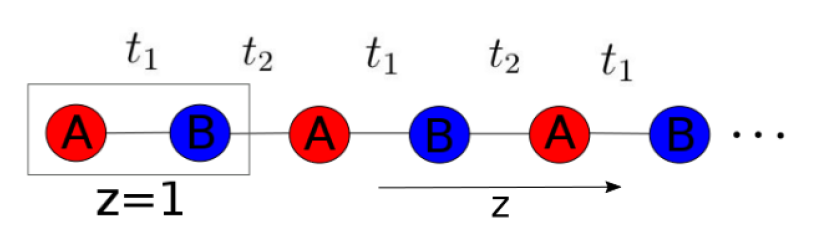
\includegraphics[width=0.8\textwidth]{shockley.png}
   \caption{Modelo de Shockley 1D. La celda unitaria está representada por el rectángulo gris, y la coordenada de celda unitaria se denota por $z$. Las amplitudes de salto intra- e inter-celda se denotan por $t_1$ y $t_2$, respectivamente. Tomada de [2].}
\end{figure}

Si ambos hoppings son mayores que cero, los electrones vivirán en ambos sitios de la red, por lo tanto disminuyendo su energía cinética. El Hamiltoniano correspondiente puede ser escrito en segunda cuantización como
\begin{equation}
H = \sum_z \Psi^{\dagger}(z)\left[U\Psi(z)+V\Psi(z-1)+V^{\dagger}\Psi(z+a)\right],     
\end{equation}
donde 
\[U=
\begin{pmatrix}
0 & t_1^{\*} \\
t_1 & 0 
\end{pmatrix}, \ \ \ \ 
V=
\begin{pmatrix}
0 & t_2^{\*} \\
0 & 0 
\end{pmatrix},
\]
donde $t_1$ y $t_2$ son las amplitudes de tunelaje intra- e inter-celda, respectivamente, $z$ es la coordenada de celda unitaria y $\Psi(z)$ es el espinor
\begin{equation}
    \Psi(z)=\begin{pmatrix}
\Psi_a(z) \\
\Psi_b(z) 
\end{pmatrix},
\end{equation}
cuyas componentes hacen referencia a las funciones de onda en las subredes A y B, respectivamente.\\

Es posible demostrar que haciendo una transformada de Fourier al hamiltoniano de la Eq. (1), para pasar a funciones de onda en el espacio de momentos del cristal, se obtiene el hamiltoniano
\begin{equation}
    H(k)= \begin{pmatrix}
    o & t^{*}\\
    t(k) & 0
    \end{pmatrix}, \ \ \ \ t(k)\equiv t_1 + t_2 e^{ik} = t_1 + qt_2.
\end{equation}
Resolviendo la ecuación de Scr\"odinger para este hamiltoniano resulta en las eigenenergías y eigenfunciones
\begin{equation}
    E(k)= \pm \sqrt{t_1^2 + t_2^2 + 2t_1 t_2\mathrm{cos}(k)},\ \ \ \Psi(k) = \frac{1}{\sqrt{2}}
    \begin{pmatrix}
    e^{i\mathrm{arg}[t(k)]} \\
    \pm 1
    \end{pmatrix},
\end{equation}
que corresponde a bandas de energía simétricas correspondientes al par partícula-hueco (Fig. 2 (arriba)).\\

Para analizar los estados de borde se introduce un corte en la cadena 1D y se considera a esta como semi-infinita (Fig. 1). Esto corresponde a un corte en la unión $t_2$, por lo que se expone un átomo A en el borde. De la Ec. (4) se puede observar que para cualquier par de valores $t_1$, $t_2$ existe un valor $k_0$ tal que $E(k_0)=0$, es decir, se activa el modo cero de energía (para $t_1=t_2$ se tiene $k_0=\pi$), esto deriva en la relación para los hoppings
\begin{equation}
    q_0=-\frac{t_1}{t_2}.
\end{equation}
Se puede obtener la eigenfunción para la subred A, $\psi_a(z)=q_0^{z-1}$, de donde se observa que, para que cumpla con la condición de que se desvanezca en infnito, se debe cumplir
\begin{equation}
|q_0=\frac{|t_1|}{|t_2|} < 1,
\end{equation}
relación que se conoce como criterio de Shockley: \textit{En el modelo de tight-binding 1D con amplitudes de tunelaje alternates, el estado de borde existe si el hopping con mayor magnitud se rompe en la frontera}. Este criterio se observa más fácilmente por medio de una cantidad denominada ``winding number'' ($W$), definida como
\begin{equation}
    W= \frac{1}{2\pi i} \oint_C dq \frac{d}{dq} \mathrm{ln} [t(q)],
\end{equation}
el cual tiene la propiedad de que si $t(q_0)=0$ se encuentra dentro del contorno $C$ definido por $t(k)$ entonces se obtiene $W=1$, de otra forma $W=0$. En otras palabras, si $|t_2|< |t_1|$ el contorno no alcanza el orígen, lo cual es requerido para la existencia de estados de borde (Fig. 2 (abajo)).\\

\begin{figure}[th!]
   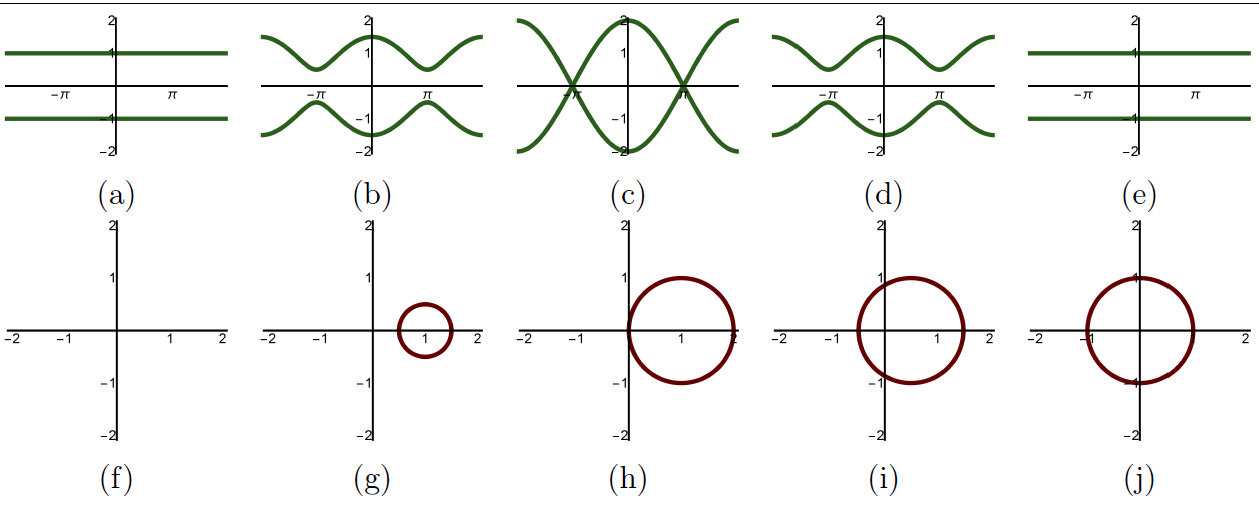
\includegraphics[width=0.97\textwidth]{bandas_shockley.png}
   \caption{(arriba) Relación de dispersión para el modelo de Shockley 1D para los casos: (a) $t_1=1$, $t_2=0$, (b) $t_1=1$, $t_2=0.5$, (c) $t_1=1$, $t_2=1$, (d) $t_1=0.5$, $t_2=1$, (e) $t_1=0$, $t_2=1$. (abajo) Respectivas graficas de contorno de $t(k)$ conforme $k$ barre la zone de Brillouin ($0$ a $2\pi$) para los casos (a)-(e). Tomada de [2].}
\end{figure}

Esto se resume en el resultado
\begin{equation}
    W= \begin{cases} 
0 \ \ \mathrm{No\ existe\ estado\ de\ borde}\ (|t_2|< |t_1|), \\
1 \ \ \mathrm{Existe\ estado\ de\ borde}\ \ \ \ \ (|t_2|\geq |t_1|).
\end{cases}
\end{equation}
A continuación se muestran algunas NNs implementadas para este sistema.

\subsection{Implementación de NNs}
Se procedió a implementar algunas NNs sobre el modelo de Shockley. El primer caso aprende a diferenciar una fase topológica trivial (T), esto es, no estados de borde, de una no trinial (NT) en donde existen estados de borde, a partir del valor de los hoppings $t_1$ y $t_2$. El segundo caso realiza la misma tarea pero ahora a partir de imágenes de las gráficas de contorno de $t(k)$.

\subsubsection{T o NT a partir de hoppings}
En este caso se trata de que la NN aprenda a diferenciar entre T y NT a partir de una base de datos con diferentes valores de los hoppings. Para ello, se generó una base de datos almacenada en un archivo csv con las columnas "T", "t1", "t2", además de una columna al inicio indicando la fila de los datos. La primera columna, que representa el label, está representada por ceros y unos (NT y T), respectivamente. Las columnas dos y tres están representadas por los valores reales de los hoppings, barriendo $t_1$ y $t_2$ de cero a uno con un intervalo de 0.005, teniendo así un set de datos de tamaño 40401  (Fig. 3). Este tamaño se divide en un set de entrenamiento y un set de validación con 0.8 y 0.2 porciones del set total, respectivamente.  

\begin{figure}[th!]
\centering
   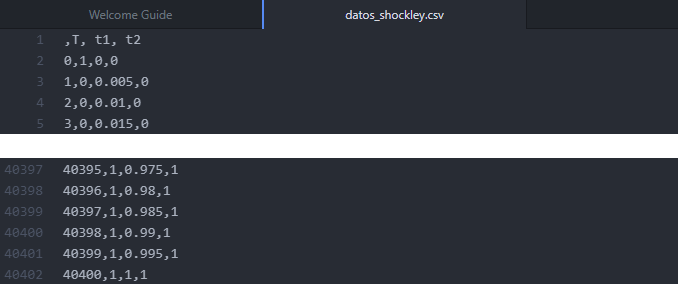
\includegraphics[width=1.\textwidth]{datos_shockley.png}
   \caption{Base de datos utilizada para la NN.}
\end{figure}

Como se observa en la Fig. 7 en el Apéndice, el modelo alcanza una exactitud del $99.72\%$ después de 60 épocas de entrenamiento, y una exactitud del $99.63\%$ para el set de validación, por lo que puede decirse que la NN ha logrado aprender y es capaz de predecir con gran exactitud.

\subsubsection{T o NT a partir de imágenes de contorno de $t(k)$}
En este caso se trata de que la NN aprenda a diferenciar entre T y NT a partir de una base de datos con imágenes de contorno de $t(k)$ (como por ejemplo las Figs. 2(f-j)). Para ello, se generó una base de datos almacenada en un archivo csv con las columnas "file\_name" y "label" (Fig. 4). La primera columna contiene el nombre de las imágenes que se utilizan en la NN, mientras que la segunda columna, que representa el label, está representada por ceros y unos, haciendo referencia a NT y T, respectivamente. 

\begin{figure}[th!]
\centering
   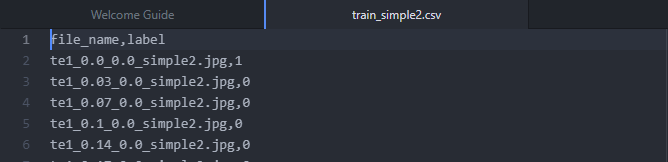
\includegraphics[width=1.\textwidth]{datos_imagenes_shockley.png}
   \caption{Base de datos utilizada para la NN.}
\end{figure}

Se generaron 900 imágenes barriendo $t_1$ y $t_2$ de cero a uno con un intervalo de 0.033. Cada imágen tiene dimensión de $128\times128$ pixeles con escale de colores \textit{grayscale}. En la Fig. 5 se observan algunas de las imágenes que se utilizaron en el entrenamiento de la NN.

\begin{figure}[th!]
\centering
   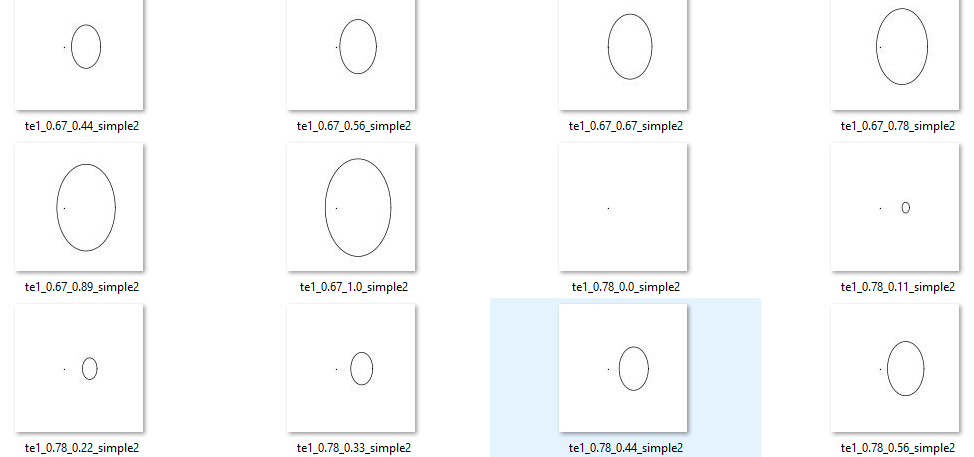
\includegraphics[width=1.\textwidth]{imagenes_shockley.png}
   \caption{Ejemplos de imágenes utilizadas para la NN.}
\end{figure}

Como se observa en la Fig. 8 en el Apéndice, el modelo alcanza una exactitud del $99.11\%$ después de solo 10 épocas de entrenamiento, y una exactitud del $90.0\%$ para el set de validación, por lo que, al igual que en el caso anterior, la NN es capaz de identificar fases topológicas no triviales como se deseaba.

\section{Implementación de NNs en grafeno con/sin impurezas}
Una vez que adquirimos algo de experiencia con el modelo de Shockley, se procedió a utilizar NNs para la predicción de algunas propiedades del modelo en estudio. A continuación se presentan los modelos de NN que se implementaron para grafeno:
\begin{itemize}
    \item Clasificación en I o NI a partir de $j$ y $F_D$.
    \item Para el caso de una sola impureza, inferir el radio ($R$) de esta a partir de $F_D$.
    \item Generalizando el caso anterior, para 1, 2 o 3 impurezas en serie (todas con el mismo radio), inferir $R$ a partir de $F_D$, $j$ y $N$.
    \item Variando el caso anterior,  inferir $N$ a partir de $F_D$, $j$ y $R$.
\end{itemize}

Para todos los casos se utilizó el mismo set de datos mostrado en la Fig. 6, tomando en cada NN las columnas necesarias en cada caso.

\begin{figure}[th!]
\centering
   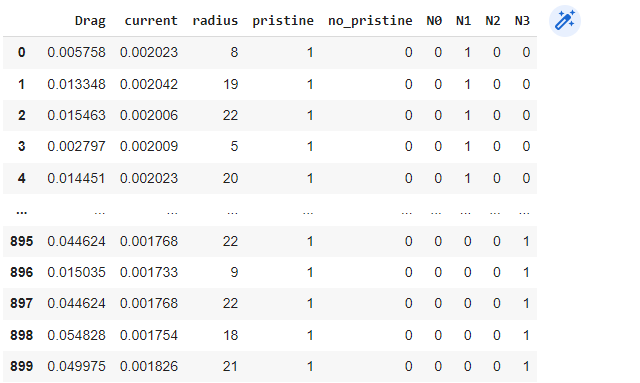
\includegraphics[width=1.\textwidth]{datos_grafeno.png}
   \caption{Base de datos utilizada para las NNs en grafeno.}
\end{figure}

El set de datos, archivo csv, contiene un total de 1200 filas (300 para 0 impurezas, 300 para 1 impureza, 300 para 2 impurezas y 300 para 3 impurezas), cada una con los datos (columnas): \textbf{Drag}, que representa el valor de la fuerza de arrastre ($F_D$); \textbf{current}, que dennota la densidad de corriente eléctrica ($j$), la cual es calculada en el punto $(11N_x/12, N_y/2)$, donde $N_x$ y $N_y$ representan el tamaño de la red; \textbf{radius}, que representa el tamaño del radio ($R$, que adquiere valores aleatoriamente entre 2 y 25) de la(s) impureza(s) colocada(s) en el sistema de grafeno, donde la ubicación del centro de cada impureza se coloca con coordenadas ($x_i=\frac{N_x(i+1)}{N +1}$, $y_i=\frac{N_y}{2}$), donde $N$ es el número de impurezas colocadas en el sistema (todas con el mismo $R$); \textbf{pristine}, que hace referencia a si el sistema contiene (1) o no contiene (0) impurezas, el cual se encuentra \textit{one-hot encoded}, es decir, se separa en varias columnas (dos en este caso) representando cada posible valor de la columna original; finalmente se tienen las (one-hot encoded) columnas correspondientes al número de impurezas colocadas en el sistema \textbf{N}. Dicho set de datos se obtuvo del RLBM 2D que ya tenemos implementado (revisar reportes anteriores) para grafeno, utilizando los parámetros: $N_x =512$; $N_y=128$; $N_{steps}=1024$; $\delta_t=1$; se utilizaron Condiciones de Frontera (BC's) periódicas en los bordes inferior y superior, abiertas en los bordes izquierdo y derecho, y \textit{Bounce Back} (BB) en la frontera de las impurezas sólidas; se utilizaron los parámetros $\rho_c=1.0$ (densidad de corriente), $\rho_E=0.75$ (densidad deenergía), $v_x=0.002$ (velocidad en dirección $x$), $v_y=0.0$ (velocidad en dirección $y$). A continuación se muestran los resultados de cada caso implementado. 

\subsection{¿Con impureza (I) o sin impureza (SI)?}
En primer lugar, partiendo del caso mas sencillo, se creó una NN con el propósito de identificar si la red de grafeno contiene alguna impureza en su interios o si no existen impurezas (caso pristino) a partir de los valores de $j$ y de $F_D$. Para este caso se utilizó como \textit{features} a las primeras dos columnas del set de datos de la Fig. 6 y como \textit{label} o resultado los valores de las columnas 4 y 5. Este set de datos elegido se divide en un set de entrenamiento y un set de validación con 0.8 y 0.2 porciones del set total, respectivamente.\\

Como se observa en la Fig. 10 en el Apéndice, el modelo alcanza una exactitud del $100\%$ después de 100 épocas de entrenamiento, al igual que para el set de validación, lo cual nos indica que la NN ha sido capaz de aprender a identificar entre las fases de manera sencilla.

\subsection{Predicción del radio de una impureza basandonos en $F_D$ y $j$}
Enseguida, considerando una sola impureza en el sistema de grafeno, se implementó una NN con el objetivo de predecir el radio de dicha impureza basándonos en los valores de $F_D$ y $j$, por lo que los features fueron nuevamente la primera y segunda columna del set de datos de la Fig. 6, mientras que los labels correspondieron a la tercera columna.\\ 

Como se observa en la Fig. 11 en el Apéndice, el modelo alcanza una exactitud del $98.16\%$ después de 600 épocas de entrenamiento, y una exactitud del $98.36\%$ para el set de validación, lo cual nos indica que la NN ha aprendido con buena precisión.

\subsection{Predicción del radio de las impurezas basandonos en $F_D$, $j$ y $N$}
También, generalizando al caso anterior, se implementó una NN con el objetivo de predecir el radio de varias (1-3) impurezas iguales basándonos en los valores de $F_D$, $j$ y $N$. En este caso los features fueron la primera y segunda columna, además de las columnas 6-9 del set de datos de la Fig. 6, mientras que los labels correspondieron a la tercera columna.\\ 

Como se observa en la Fig. 12 en el Apéndice, el modelo alcanza una exactitud del $95.38\%$ después de 600 épocas de entrenamiento, y una exactitud del $94.95\%$ para el set de validación, lo cual resulta ser un resultado bastante preciso, aunque con posibilidades de mejora.

\subsection{Predicción del numero de impurezas basandonos en $F_D$, $j$ y $R$}
Finalmente, dándole una variante al caso anterior, se implementó una NN con el objetivo de predecir el número de impurezas colocadas en el sistema de grafeno basándonos en los valores de $F_D$, $j$ y $R$. En este caso los features fueron las primeras tres columnas del set de datos de la Fig. 6, mientras que los labels correspondieron a las columnas 6-9.\\ 

Como se observa en la Fig. 13 en el Apéndice, el modelo alcanza una exactitud del $99.27\%$ después de 100 épocas de entrenamiento, y una exactitud del $99.58\%$ para el set de validación, lo cual resulta ser un resultado bastante preciso.\\

Cabe señalar que en todos los casos se implementó también la NN sin tomar en cuenta a $j$ dentro de los features, y el resultado fué bastante similar en cuanto a precisión, sin embargo al modelo le toma más tiempo el aprendizaje, como es de esperarse.

\section{Trabajo en proceso y a futuro}
Actualmente me encuentro trabajando en la implementación de campos externos dentro de la red de grafeno en el RLBM 2D, para lo cual se debe realizar un análisis teórico de los cambios de su implementación del caso clásico al relativista. Si somos capaces de incluir dichos efectos de campos externos, se podrían incluir tanto estos parámetros, como tal vez la fuerza de sustentación, además de algunos otros parámetros de reelevancia en el sistema, en el trabajo de clasificación de sistemas por medio de NNs, lo cual nos podría servir para describir y predecir algún fenómeno conocido en el transporte en grafeno. Además, voy a comenzar a estudiar más a fondo otro tipo de sistemas de estado sólido, como son los aislantes topológicos, con el propósito de tratar de describirlos desde un punto de vista tanto teórico como hidrodinámico por medio del RLBM, además de poder hacer problemas de clasificación o predicción por medio de NNs. Para ello estaré cursando la materia \textit{CURSO ESPECIAL DE FÍSICA-AISLANTES TOPOLÓGICOS}. También en el sigiente semestre tomaré un curso especial sobre \textit{SUPERSIMETRÍA}, enfocado a sistemas 2D como el grafeno y otros sistemas de interés, con el fin de adquirir otras herramientas matemáticas para el tratamiento de este tipo de sistemas.  

\section{Congresos y escuelas}
Es adecuado comentar que durante el periodo que comprende al semestre que concluyó, se tuvo la participación como \textbf{Moderador} en la mesa de diálogo “\textit{¿Qué es la física de partículas?}” dentro
del marco de la \textbf{SEMANA DE DIVULGACIÓN DE LA FÍSICA} llevada a cabo el día 22 de Junio del 2022.


\section*{Bibliografía}
[1] D. Carpentier and L. Lévy, \textit{Aislantes topológicos}, Investigación y ciencia \textbf{467} (2015) 75-83. \newline
[2] J. K. Asbóth, L. Oroszlány and A. Pályi, \textit{A short course on topological insulators}, (Springer, Lecture notes in Physics, 2016). \newline
[3] P. R. Beresford Tunstall, \textit{The Shockley model for topological insulators}, Bachelor's thesis, University of Copenhagen (2016).
\newpage

\section*{Apéndice: códigos de implementación de las NNs en TensorFlow}
A continuacón se muestran los códigos para cada NN implementada. Para el caso de grafeno, los cuatro programas tienen como códgo inicial el mostrado en la Fig. 9, cambiando únicamente las lineas 22 y 23 en donde se eligen las columnas para el entrenamiemto en cada caso.
\begin{figure}[th!]
\centering
   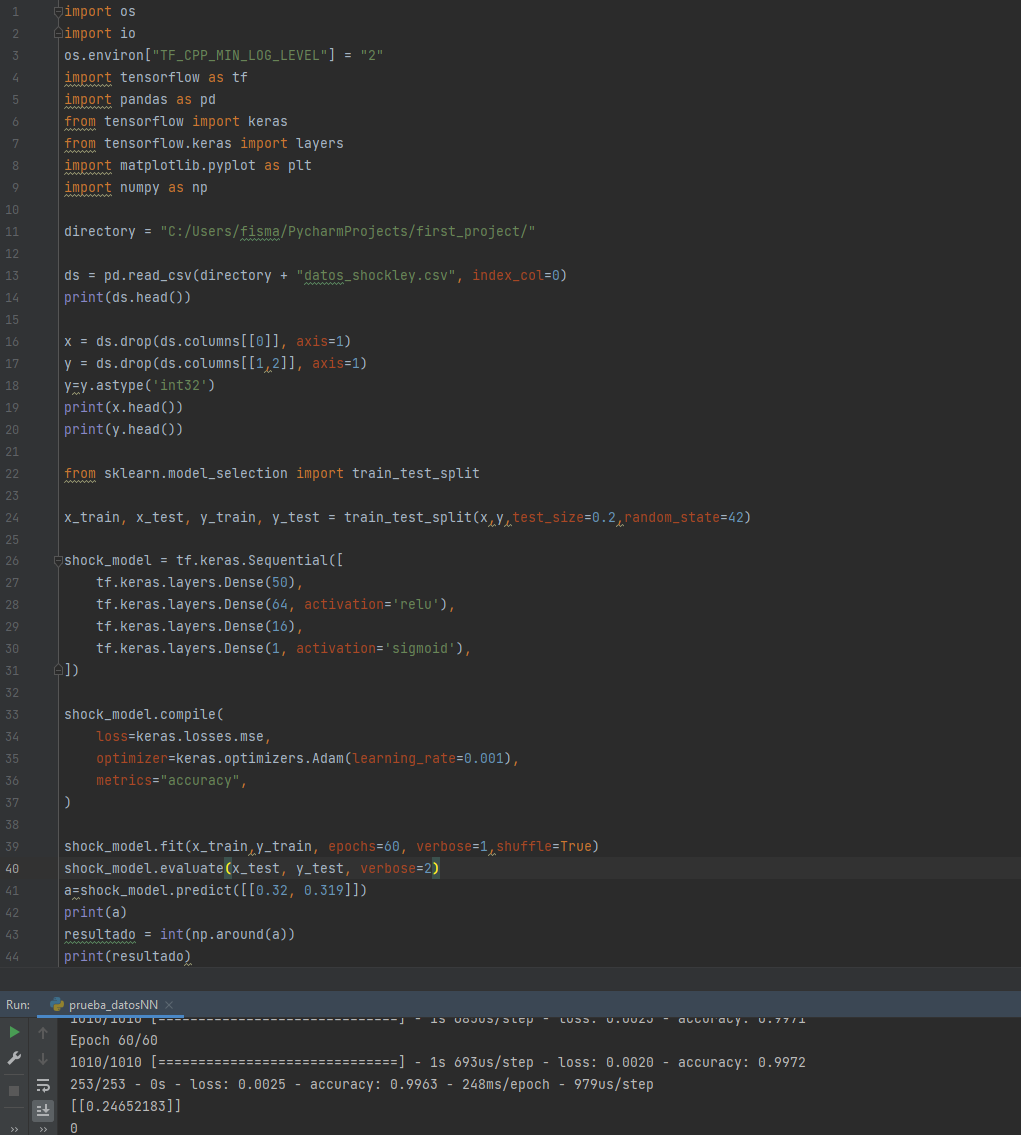
\includegraphics[width=1.\textwidth]{prog_shockley_datos.png}
   \caption{Código de NN para el la predicción T/NT basado en $t_1$ y $t_2$.}
\end{figure}
\newpage
\begin{figure}[th!]
\centering
   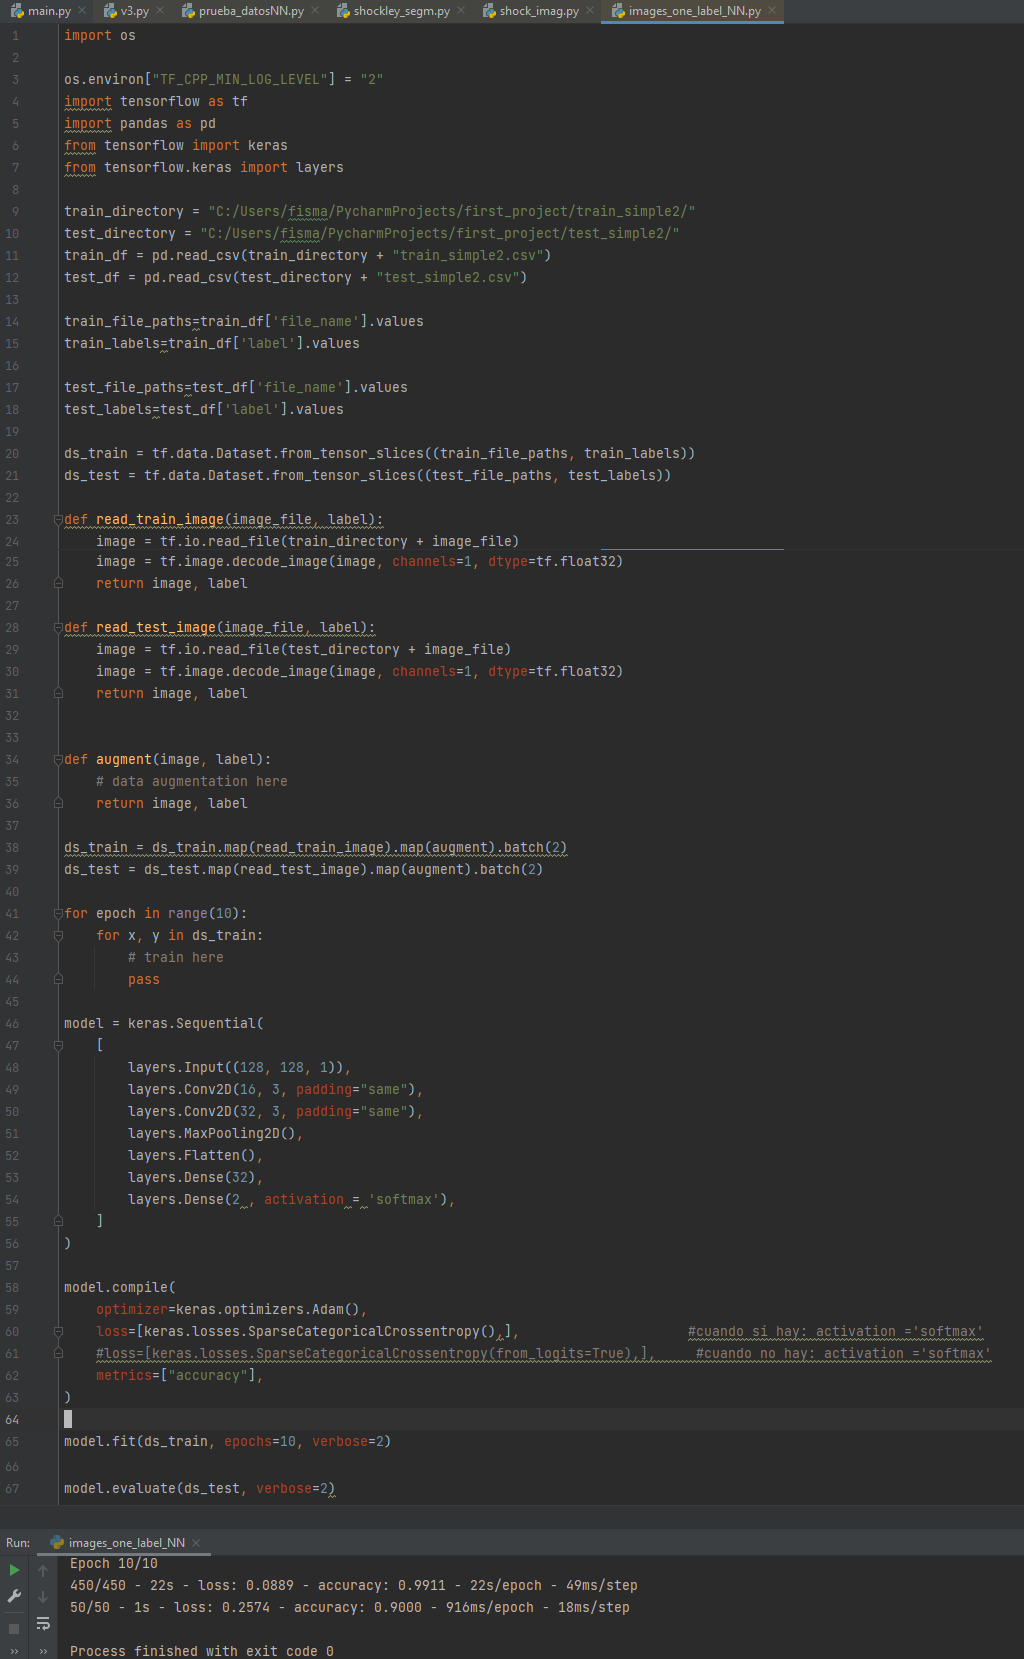
\includegraphics[width=1.\textwidth]{prog_imagenes_shockley.png}
   \caption{Código de NN para el la predicción T/NT basado en la gráfica de contorno de $t(k)$.}
\end{figure}
\begin{figure}[th!]
\centering
   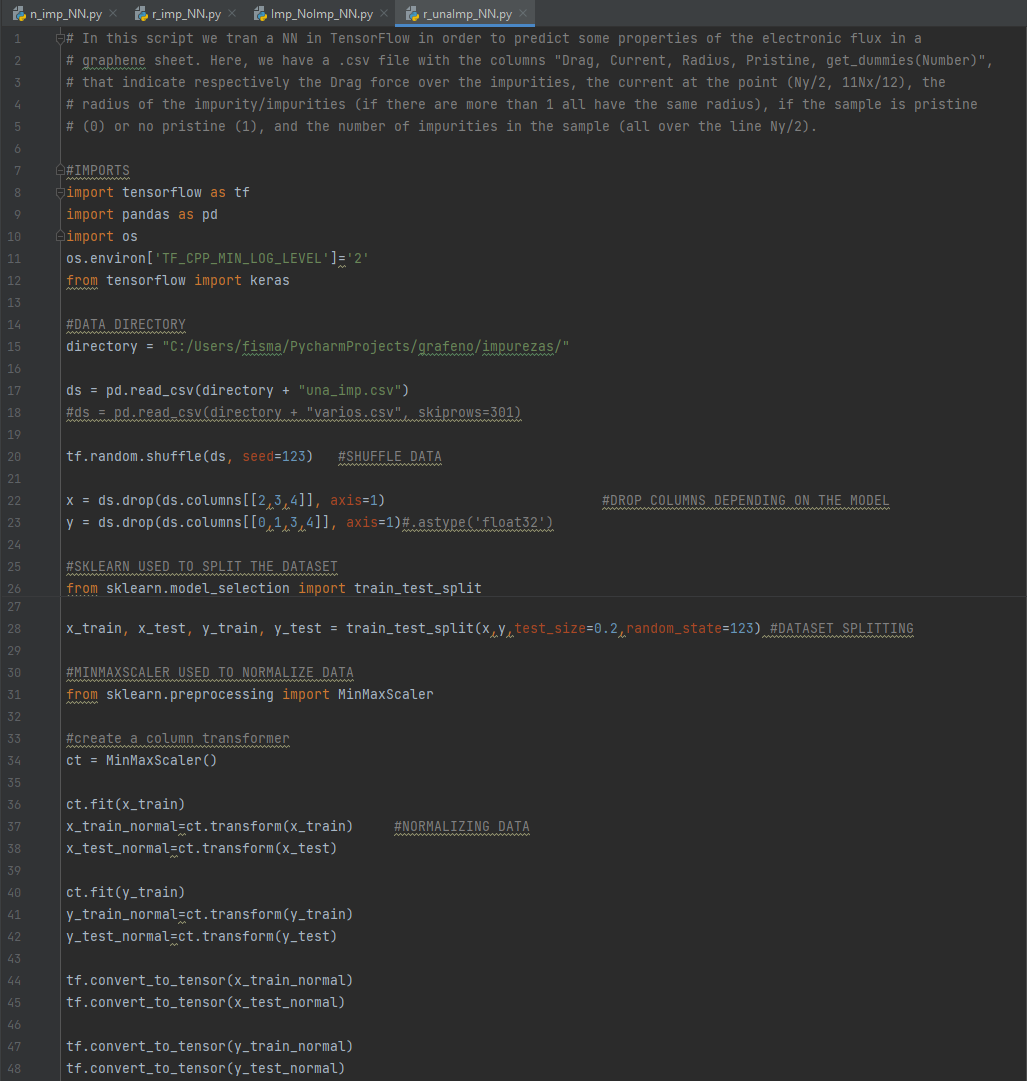
\includegraphics[width=1.\textwidth]{prog_grafeno.png}
   \caption{Código de importación y tratamiento de set de datos para las NNs en grafeno.}
\end{figure}
\begin{figure}[th!]
\centering
   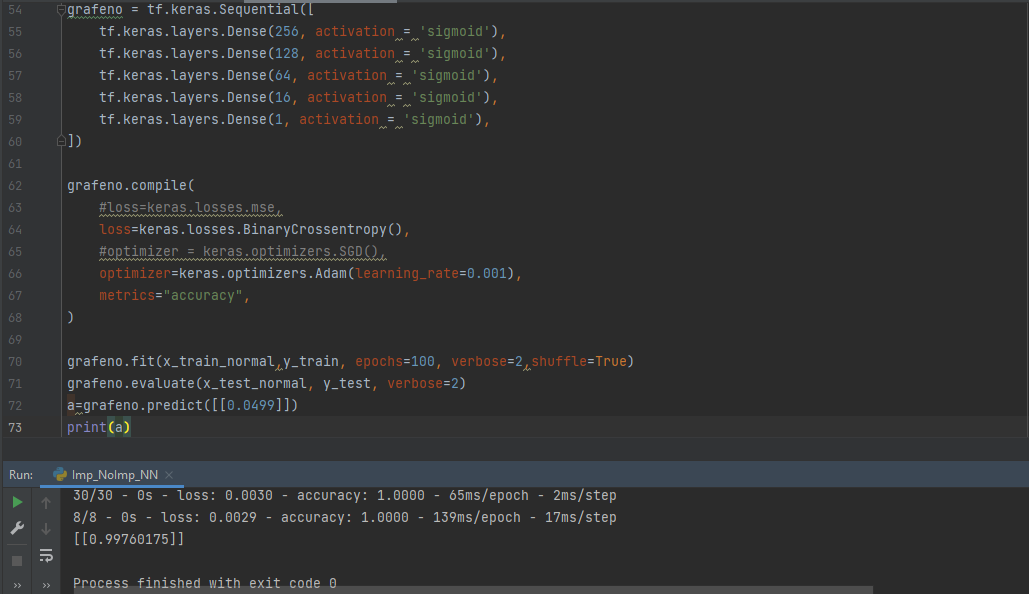
\includegraphics[width=1.\textwidth]{I_NI_NN.png}
   \caption{Código de NN para el la predicción de Pristine/NoPristine basado en $F_D$ y $j$.}
\end{figure}
\begin{figure}[th!]
\centering
   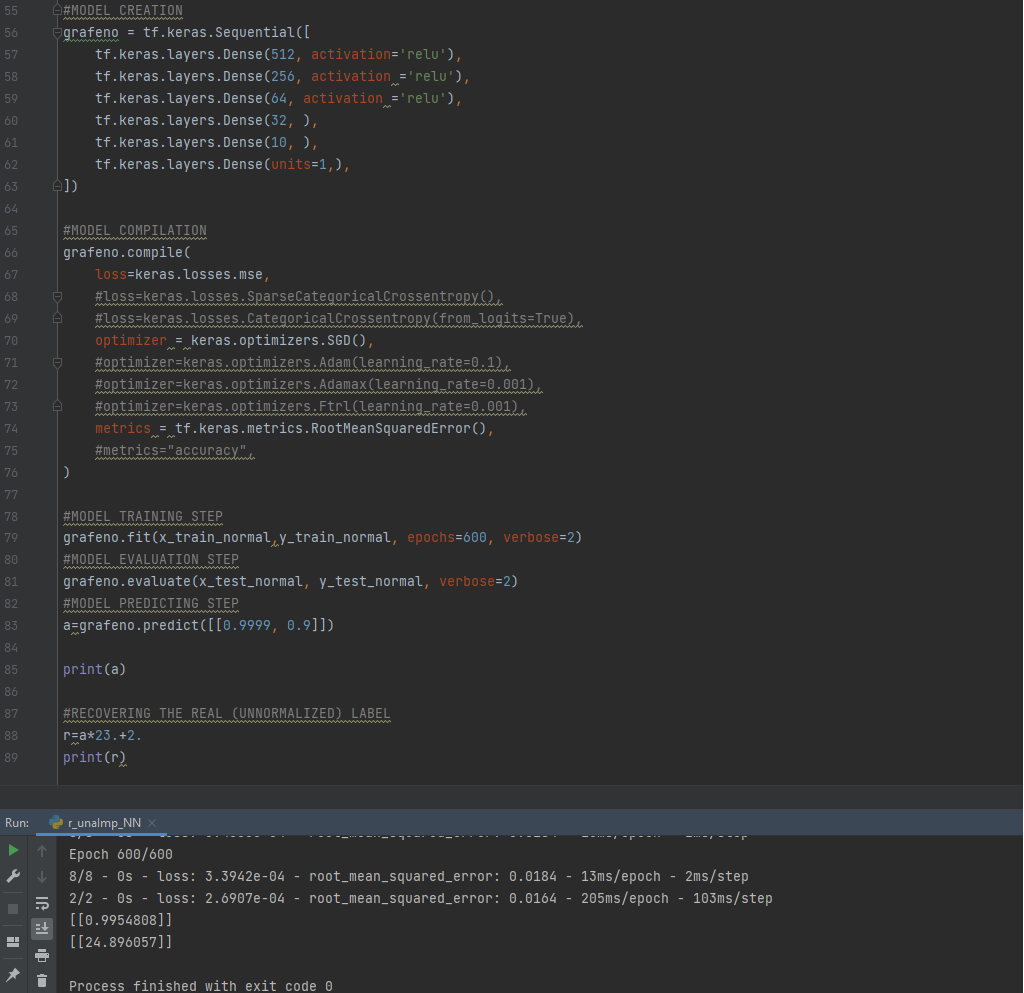
\includegraphics[width=1.\textwidth]{unaImp_NN.png}
   \caption{Código de NN para el la predicción de $R$ basado en $F_D$, $j$ para una impureza.}
\end{figure}
\begin{figure}[th!]
\centering
   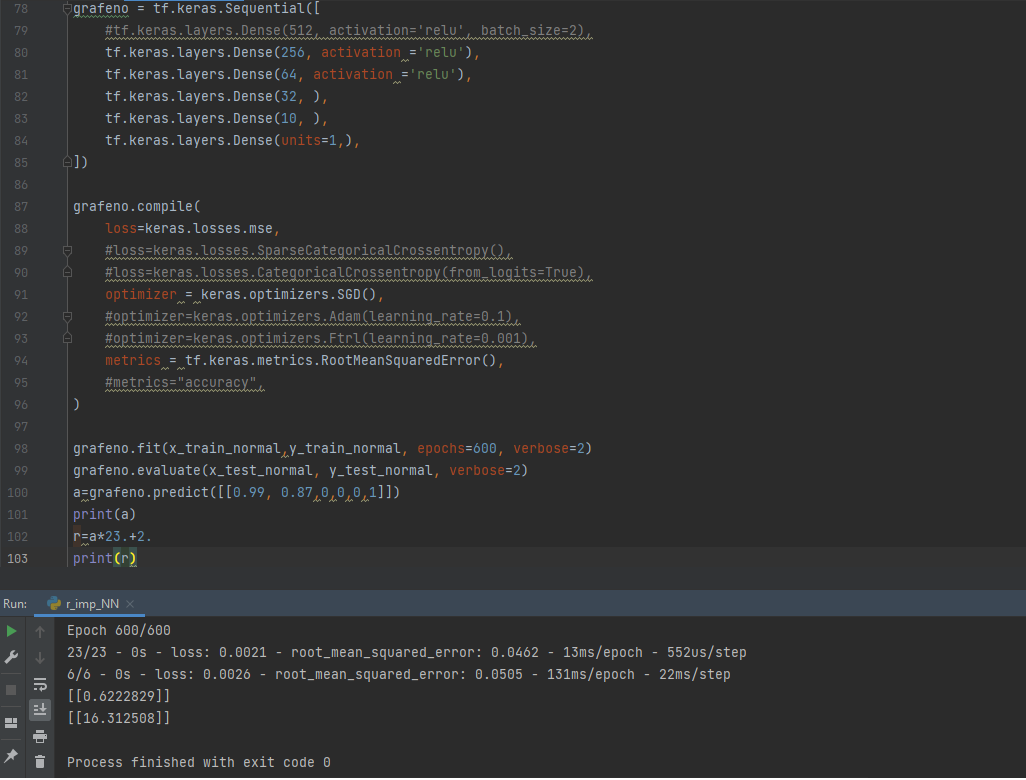
\includegraphics[width=1.\textwidth]{r_Varias.png}
   \caption{Código de NN para el la predicción de $R$ basado en $F_D$, $j$ y $N$ para varias impurezas.}
\end{figure}
\begin{figure}[th!]
\centering
   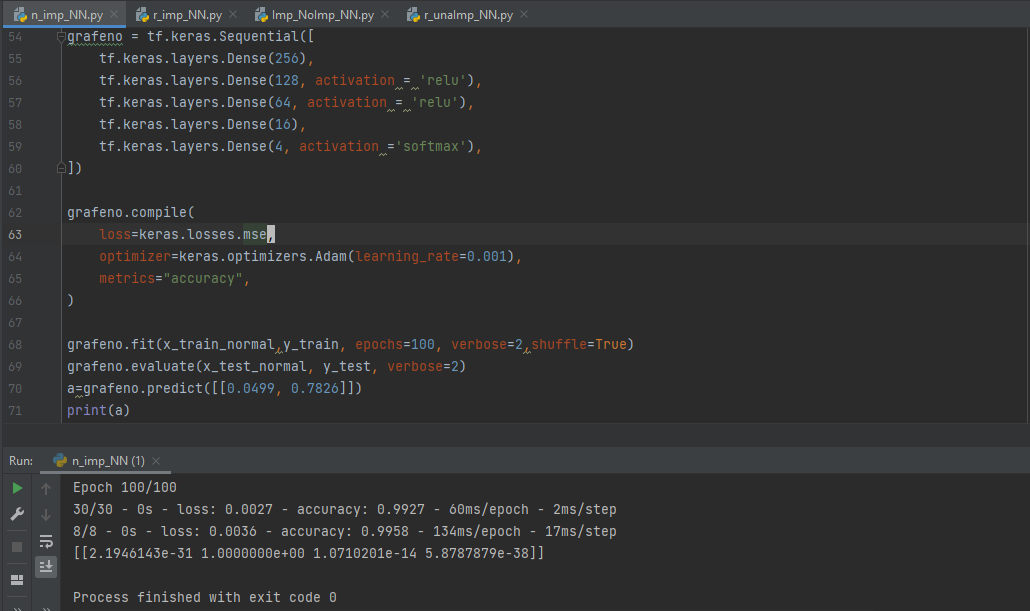
\includegraphics[width=1.\textwidth]{n_Varias.png}
   \caption{Código de NN para el la predicción de $N$ basado en $F_D$, $j$ y $R$ para varias impurezas.}
\end{figure}

\end{document}